\section{Introducción}
Las ecuaciones diferenciales de primer orden aparecen en una gran variedad de problemas del mundo real. 
Se utilizan para modelar fenómenos en la física, biología, economía, ingeniería y otras disciplinas.
En este capítulo, se explorarán diversas aplicaciones del modelado con ecuaciones diferenciales de primer orden.


\section{Interés Compuesto Continuo}

Una persona deposita \$5000 en su cuenta con interés compuesto continuo. Suponiendo que no hay depósitos adicionales ni retiros, ¿cuánto dinero habrá en la cuenta después de 7 años si la tasa de interés es constante del 8.5\% durante los primeros 4 años y del 9.25\% durante los últimos 3 años?

La fórmula del interés compuesto continuo es:

\[
P = A e^{kt}
\]

Dado que inicialmente el monto es:

\[
P_0 = 5000, \quad t_0 = 0
\]

Determinamos el modelo inicial:

\[
5000 = A e^{k(0)}
\]

\[
A = 5000
\]

Sustituyendo en la fórmula:

\[
P_1 = 5000 e^{kt}
\]

Para los primeros 4 años, con \( k = 0.085 \):

\[
P_1 = 5000 e^{0.085(4)}
\]

\[
P_1 = 7024.74
\]

Para los siguientes 3 años, usamos la misma ecuación:

\[
P_2 = A e^{0.0925 t}
\]

En el punto de 4 años, recalculamos \( A \):

\[
P_2 = 7024.74, \quad t_2 = 4
\]

\[
7024.74 = A e^{0.0925(4)}
\]

\[
A = \frac{7024.74}{e^{0.0925(4)}} = 4852.23
\]

Por lo tanto, la solución a la ecuación diferencial bajo estas condiciones es:

\[
P_2 = 4852.23 e^{0.0925 t}
\]

Para calcular el monto en el año 7:

\[
P_2 = 4852.23 e^{0.0925(7)}
\]

\[
P_2 = 9271.44
\]

\subsection{Representación Gráfica}
\noindent
\begin{figure}[H]
    \centering
    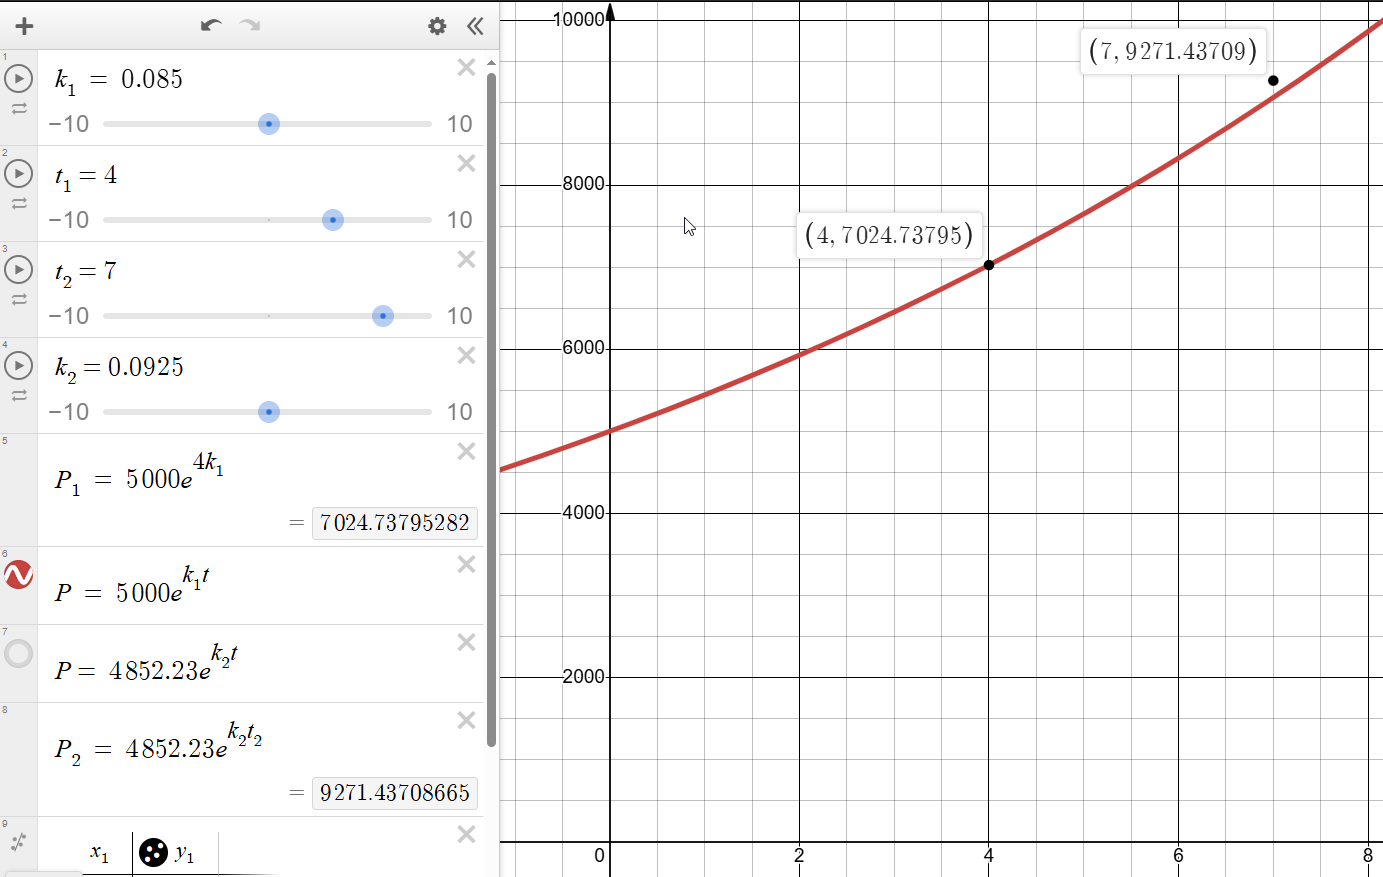
\includegraphics[width=0.6\textwidth]{images/Modelado 01.png}
    \caption{Modelo de interés compuesto continuo}
    \label{fig:modelo-interes}
\end{figure}


\section*{Ejercicio 1: Crecimiento de una Población de Bacterias}

Un determinado estudio de bacterias inicialmente tiene una población \( P_{0} \). Tras haber transcurrido 1 hora, el número de bacterias aumentó a \( \frac{3}{2} P_{0} \). 

Si la tasa de crecimiento es proporcional al número de bacterias presentes en un tiempo \( t \), determina el tiempo necesario para que la población de bacterias triplique su valor.

\begin{figure}[H]
    \centering
    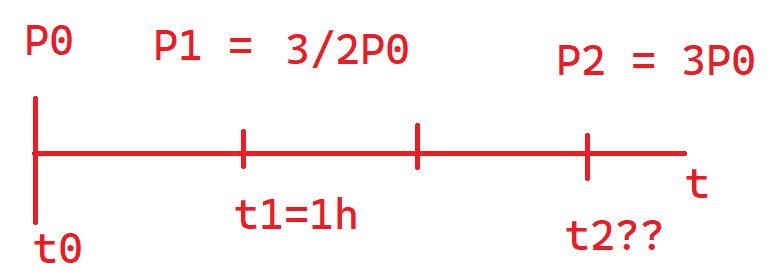
\includegraphics[width=0.7\textwidth]{images/Modelado 02.png}
    \caption{Representación del problema de crecimiento bacteriano}
\end{figure}

La ecuación diferencial que modela el problema es:

\[
\frac{dP}{dt} = kP
\]

Resolviendo:

\[
\int \frac{1}{P} dP = \int k dt
\]

\[
\ln(P) = kt + c
\]

\[
P = e^{kt+c}
\]

\[
P = A e^{kt}, \quad \text{donde } A = e^c
\]

Utilizando los datos iniciales:

\[
P(0) = P_{0} \Rightarrow P_{0} = A e^{k(0)}
\]

\[
A = P_{0}
\]

Para \( P(1) = \frac{3}{2} P_{0} \):

\[
\frac{3}{2} P_{0} = P_{0} e^{k(1)}
\]

\[
\frac{3}{2} = e^k
\]

\[
k = \ln\left(\frac{3}{2}\right) = 0.40
\]

Para determinar \( t_2 \) donde \( P(t_2) = 3P_{0} \):

\[
3 P_{0} = P_{0} e^{0.4t_{2}}
\]

\[
3 = e^{0.4t_{2}}
\]

\[
t_{2} = \frac{\ln(3)}{\ln\left(\frac{3}{2}\right)} = 2.71
\]

Si la población inicial fuera 100 bacterias:

\begin{figure}[H]
    \centering
    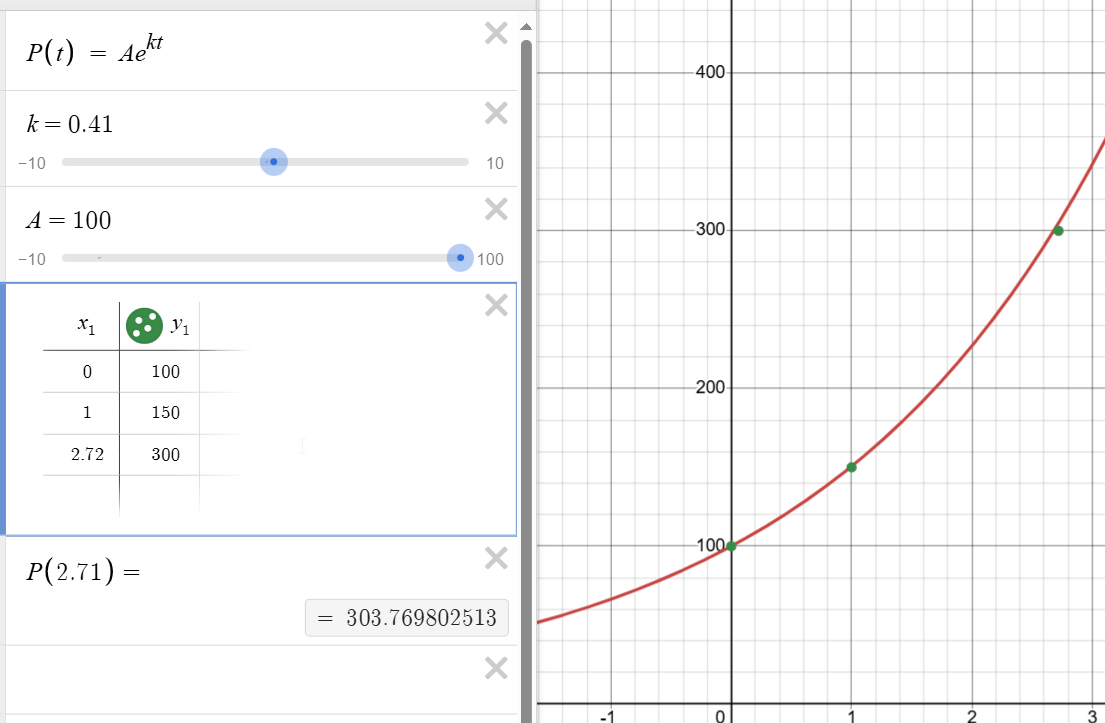
\includegraphics[width=0.7\textwidth]{images/Modelado 03.png}
    \caption{Simulación con población inicial de 100}
\end{figure}

---

\section*{Ejercicio 2: Crecimiento de una Colonia de Bacterias}

Se sabe que inicialmente la población era de 1000 bacterias y que tras 1 hora se duplicó. Se pide:

1. Determinar la ecuación diferencial particular.
2. Calcular la población tras 1.5 horas.

\begin{figure}[H]
    \centering
    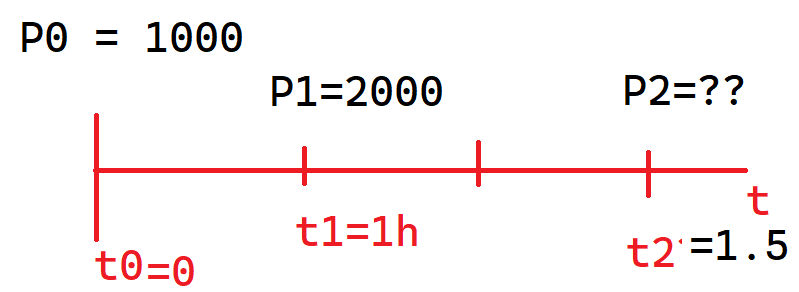
\includegraphics[width=0.7\textwidth]{images/Modelado 04.png}
    \caption{Representación del problema de crecimiento bacteriano}
\end{figure}

Datos:

\[
P(0) = 1000, \quad P(1) = 2000
\]

Usando la ecuación:

\[
P(t) = A e^{kt}
\]

\[
1000 = A e^{k(0)}
\]

\[
A = 1000
\]

\[
2000 = 1000 e^{k(1)}
\]

\[
2 = e^k \Rightarrow k = \ln(2)
\]

\[
P(t) = 1000 e^{\ln(2) t}
\]

Para \( P(1.5) \):

\[
P(1.5) = 1000 e^{\ln(2)(1.5)}
\]

\[
P(1.5) = 2828
\]

---

\section*{Ejercicio 3: Decaimiento Radioactivo}

Un material radioactivo pierde masa de manera proporcional a su cantidad presente. Se sabe que inicialmente había 50 mg y que tras 2 horas perdió el 10\% de su masa. Se pide:

1. Determinar una ecuación para la masa remanente.
2. Calcular la masa tras 4 horas.
3. Encontrar el tiempo en que la masa se reduce a la mitad.

\begin{figure}[H]
    \centering
    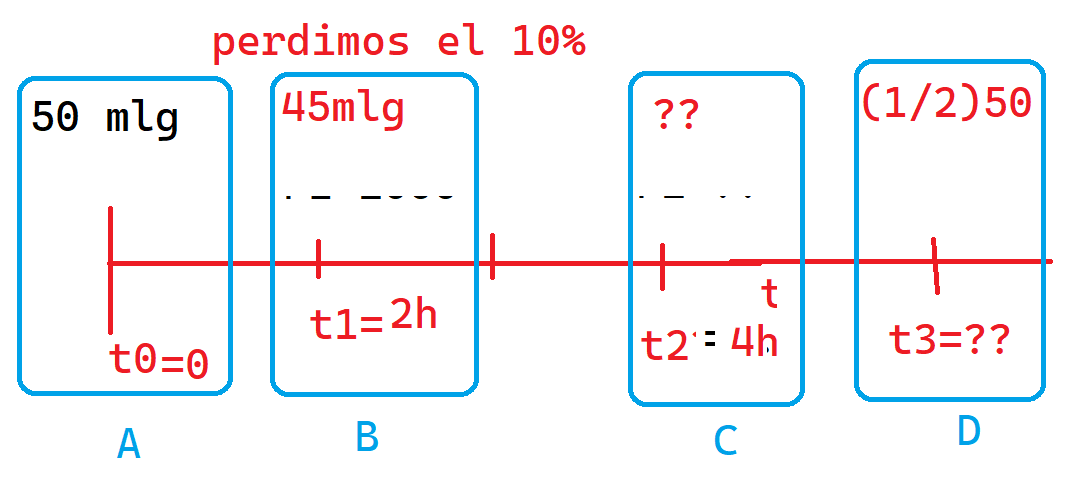
\includegraphics[width=0.7\textwidth]{images/Modelado 05.png}
    \caption{Curva de decaimiento del material radioactivo}
\end{figure}


\section*{Ejercicio 4: Enfriamiento de una Barra de Metal}

Una barra de metal con temperatura inicial de 100ºF es colocada en un ambiente con temperatura constante de 0ºF. Después de 20 minutos, su temperatura se reduce a 50ºF. Se pide:

1. Determinar el tiempo para alcanzar 25ºF.
2. Calcular la temperatura tras 10 minutos.

El problema sigue la **Ley de Enfriamiento de Newton**:

\[
\frac{dT}{dt} = -k(T - T_{\infty})
\]

\section{Crecimiento Poblacional: Modelo Logístico}
El crecimiento poblacional puede modelarse mediante la ecuación diferencial:

\begin{equation}
\frac{dP}{dt} = r P \left( 1 - \frac{P}{K} \right)
\end{equation}

donde \( P(t) \) es la población en el tiempo \( t \), \( r \) es la tasa de crecimiento y \( K \) es la capacidad de carga del entorno.

\subsection*{Ejemplo 3.1: Modelado del Crecimiento Poblacional}
Supongamos que una población de conejos sigue el modelo logístico con \( r = 0.1 \) y \( K = 500 \). Si inicialmente hay 50 conejos, determinar la ecuación de crecimiento.

\subsection*{Ejercicios}
\begin{enumerate}
    \item Resolver el modelo logístico para \( r = 0.2 \), \( K = 1000 \) con una población inicial de 100.
\end{enumerate}

\section{Caída Libre con Resistencia del Aire}
La ecuación de movimiento de un objeto en caída libre con resistencia del aire es:

\begin{equation}
m \frac{dv}{dt} = mg - kv
\end{equation}

donde \( v \) es la velocidad, \( m \) la masa, \( g \) la gravedad y \( k \) el coeficiente de resistencia.

\subsection*{Ejemplo 3.2: Cálculo de Velocidad con Resistencia del Aire}
Determinar la velocidad terminal de un paracaidista de 80 kg con un coeficiente de resistencia \( k = 10 \).

\subsection*{Ejercicios}
\begin{enumerate}
    \item Resolver la ecuación de caída libre para \( k = 5 \) y \( m = 60 \).
\end{enumerate}

\section{Enfriamiento de Newton}
El modelo de enfriamiento de Newton se expresa como:

\begin{equation}
\frac{dT}{dt} = -k (T - T_a)
\end{equation}

donde \( T \) es la temperatura del objeto, \( T_a \) la temperatura ambiente y \( k \) la constante de enfriamiento.

\subsection*{Ejemplo 3.3: Enfriamiento de un Café}
Un café a 90°C se enfría en una habitación a 20°C. Si \( k = 0.02 \), encontrar la temperatura en 10 minutos.

\subsection*{Ejercicios}
\begin{enumerate}
    \item Resolver para un objeto que comienza a 100°C en un ambiente de 30°C con \( k = 0.015 \).
\end{enumerate}

\section{Crecimiento y Desintegración Radiactiva}
La desintegración radiactiva se modela como:

\begin{equation}
\frac{dN}{dt} = -\lambda N
\end{equation}

donde \( N \) es la cantidad de sustancia y \( \lambda \) la constante de desintegración.

\subsection*{Ejemplo 3.4: Desintegración del Carbono-14}
El carbono-14 tiene una vida media de 5730 años. Encontrar la ecuación de desintegración.

\subsection*{Ejercicios}
\begin{enumerate}
    \item Determinar la cantidad restante de una muestra de 100 mg de uranio-238 después de 1000 años.
\end{enumerate}

\section{Dinámica de Enfermedades Infecciosas}
El modelo SIR para la propagación de enfermedades es:

\begin{equation}
\frac{dS}{dt} = -\beta SI, \quad \frac{dI}{dt} = \beta SI - \gamma I
\end{equation}

donde \( S \) es la población susceptible, \( I \) la infectada, \( \beta \) la tasa de transmisión y \( \gamma \) la tasa de recuperación.

\subsection*{Ejemplo 3.5: Propagación de un Virus}
Simular una epidemia con \( \beta = 0.3 \) y \( \gamma = 0.1 \) en una población de 1000 personas.

\subsection*{Ejercicios}
\begin{enumerate}
    \item Resolver el modelo SIR con \( \beta = 0.2 \) y \( \gamma = 0.05 \).
\end{enumerate}

\section{Modelos de Interés Compuesto}
El modelo de interés compuesto se describe como:

\begin{equation}
\frac{dA}{dt} = r A
\end{equation}

donde \( A \) es la cantidad de dinero e \( r \) la tasa de interés.

\subsection*{Ejemplo 3.6: Crecimiento de una Inversión}
Calcular el crecimiento de una inversión inicial de \$1000 con \( r = 5\% \) anual.

\subsection*{Ejercicios}
\begin{enumerate}
    \item Resolver para \( r = 3\% \) con una inversión de \$5000.
\end{enumerate}

\section{Regulación de la Glucosa en la Sangre}
El modelo de control de insulina se expresa como:

\begin{equation}
\frac{dG}{dt} = -k G + I
\end{equation}

donde \( G \) es el nivel de glucosa y \( I \) la insulina inyectada.

\subsection*{Ejemplo 3.7: Control de Glucosa}
Modelar la respuesta del cuerpo a una inyección de insulina con \( k = 0.1 \).

\subsection*{Ejercicios}
\begin{enumerate}
    \item Resolver para \( k = 0.05 \) con una dosis de insulina de 10 unidades.
\end{enumerate}

